\chapter{Structural Bioinformatics of PVC Proteins}\label{structbioinfo}

\epigraph{\emph{``It is very easy to answer many of these fundamental biological questions; you just look at the thing!''}}{\textit{Richard P. Feynman}}

\section{Introduction}

As large multi-partite biological complexes, there are far too many proteins involved in the biology of PVCs to study them all, in detail, experimentally within a single project. However, due to the increasing availability of high performance computing resources, it is possible to study all the genes and proteins, to some extent and to reasonable confidence, using bioinformatics approaches, such as homology modelling, which is becoming increasingly popular as the rate of high quality genome sequences vastly outstrips the rate of experimental protein structure resolution \citep{Rodriguez1998}. This chapter attempts to glean as many clues as possible about structure and function of the proteins involved in construction of PVCs, by `brute force', with the application of techniques which have not been attempted to date.

Since there are numerous PVC operons that have been identified, and each one contains $>$16 proteins, the dataset quickly becomes unmanageable for the experimentalist. A rigorous exploration of the hypothetical structures and functions of the proteins can collapse this dataset somewhat, and reveal subtleties of the structures which are interesting or relevant for further study. 

As the databases for gene function and protein structure are continuously updated and improved, this chapter is also a `revisit' to the now outdated genome annotations that were first put together when the strains were sequenced. By re-running these analyses at various points, new putative functions and homologies may be discovered.

Furthermore, this chapter is intended to `pull double duty' somewhat; to serve both as an exploration of new roles and information regarding PVC proteins, but also as a continued, extended, introduction or `guided tour', including what is known about each of the individual proteins within the PVCs, in a similar manner to the exploration of related structures in the Introduction. Hopefully, therefore, this chapter will provide the reader with a understanding of the PVCs with regard to what is already known and what has been discovered, on an almost gene-by-gene basis.

\subsection{The sequence identity problem}
Despite progress in the elucidation of many related structures, as shown in \vref{intro}, much is still unclear with regard to PVCs. Many PVC proteins in the existing \Pa{} annotations are listed as `hypothetical', and in the case of some older genome annotations for some of the more diverse PVC elements, this can be the entire operon \citep{Duchaud2003}. The frequent lack of known good homologues from studying the genes through BLAST for instance, and the degree of sequence diversity that can be seen in the PVCs (see \vref{bioinformatics} for a more in-depth discussion), despite producing the same structure, suggested that structural studies might offer additional/better information.

It is now a widely accepted phenomenon that sequence identity cannot always provide sufficient structural understanding on its own, as the evolutionary rules that constrain structures are not exactly the same as those that constrain sequences. Consequently, protein structures are known to evolve slower than the amino acid sequence, and slower still than the nucleotide sequence. In fact, this rate of change has even been quantified, and is estimated to be between three and ten times as slow \citep{Illergard2009}. Moreover, proteins with entirely unrelated sequences can give rise to functionally equivalent proteins, meaning this analogy between proteins would be completely missed through sequence studies alone. Now, of course this does not completely devalue the position of the sequence in determining protein structure and function, however, as \cite{Illergard2009} and \cite{Chothia1986} explain, the relationship between structural similarity (as quantified by Root Mean Square Deviation (RMSD)), and sequence identity is not linear. One of the earliest papers to explore this disconnect defined a so-called `twilight zone' of structural similarity, observing that once sequence identity dropped to around 25\% and below, false positive hits begin to predominate \citep{rost1999twilight}. Just to labor the point a little further, \cite{Holm1996} explain how structures are able to remain much the same, ``even when all sequence memory appears
to have been lost". This means that for proteins whose common ancestors are extremely far back in time, it effectively becomes meaningless to compare the DNA or amino acid sequences, and only the 3D structure matters. The authors summarise this quite nicely with the analogy, 

\begin{displayquote}
``Comparing protein shapes rather than protein sequences is like using a bigger telescope that looks farther into the universe, and thus farther back in time, opening the door to detecting the most remote and most fascinating evolutionary relations."
\end{displayquote}

To make matters worse, even proteins which \emph{do} share significant sequence identity, do not necessarily have the same structure, and therefore may differ in function. A really good example of this is epitomised by the ``Paracelsus challenge". Posed by \cite{Rose1994}, the challenge was to convert one protein's conformation to that of another protein by altering less than 50\% of the sequence. This was achieved first by \cite{Dalal1997} (winning them a \$1,000 wager in the process), and though they did have to change roughly 44\% of the protein and include an additional 7 amino acids for solubility (bringing to mind a somewhat Ship-of-Theseus argument), they were able to convert an almost entirely $\beta$-sheet protein in to an entirely $\alpha$-helical one. Subsequently, their effort has been bested by the work of \cite{Alexander2007}, and thoroughly hammers home the message of ``sequence $\neq$ structure". They were able to convert domains from \emph{Streptococcus} G proteins to retain 88\% sequence identity, yet to change their fold structures, all the while keeping their ligand binding activities.

In short, there is no substitute for being able to \emph{see} the tertiary structure and individual folds for each and every protein. This is far from a solved problem however, as it currently requires exhaustive computation and experimental efforts to generate this kind of data. Protein structure simulation has advanced significantly, but is not without its flaws, and of course, the lottery that is protein structure determination via crystallography for example is an incredibly intensive process with a high failure rate. 


Finally, to underscore this idea with some relevant examples, \cite{Leiman2010} observed that ``evolutionary relationships cannot be detected in their [tailed phages] amino acid sequences", but many structural proteins of phage origin share tertiary structure folds. One rationale for this is that given the high turn over rate of phage genomes, their evolution will occur rapidly, and thus they will explore the `chemical space' rapidly also. This is combined with the fact that phages experience a multitude of evolutionary pressures, and being proteinacious entities only, they have to be particularly `inventive' when it comes to protein structure robustness. A further example from the same paper concerns the structures of the VgrG spike proteins. They are often structurally very well conserved which is usually immediately apparent on visual inspection, and yet, the sequences of certain orthologues may share $<$15\% amino acid similarity, and due to redundancy, even lower nucleotide identity. This effectively means that to try and study sequences such as these using sequence data alone would be almost indistinguishable from random noise (though it may be possible to consider small numbers of highly conserved/`privileged' sites). \cite{Silverman2012} make the same observation for the tube proteins (Hcp/TssBC and the VgrG spike).

A further complication with purely sequence based studies, for long, multicomponent operons such as the PVCs and other caudate structures, is that it seems synteny and gene copy may also be significant, potentially playing a role in how the assembly is choreographed (phage early versus late proteins for instance). Papers like that of \cite{Sarris2014}, note that while many of the gene products are identifiable between orthologous operons, the gene copy number varies, as does the syntenic arrangement. In the case of the MAC complex discussed in the first chapter, the whole complex isn't even encoded in one location in the genome \citep{Shikuma2014}. 


To summarise, this chapter looks to address this `conservation of structure not sequence' question with regard to the PVCs, and to infer from these structures in such a way as to provide lab-testable hypotheses.

\subsection*{Chapter Aims}

\begin{itemize}
	\item Complete a thorough and sensitive functional annotation of as many PVC proteins as possible.
	\item Generate structural data and compare it to known proteins.
	\item Examine any high quality simulations for physical characteristics of the PVCs.

\end{itemize}

\clearpage

\section{Experimental procedures}
Given the lack of informative annotations from existing genomes available, the first step was a deeper dive in to the orthologies for all the CDSs from 16 PVC operons. Any information that can be obtained which improves on annotations of `hypothetical protein', even if weak, might provide insights which can be used to plan experiments in future.
	 
%    	\subsection{Annotation}\label{annotation}
%    	From a previous project, a number of \Pa{} genomes were sequenced, and a number of existing sequences in NCBI were reassembled and re-annotated along with them for consistency. In all of the work conducted, we utilised the consistent, re-annotated sequences and any given locus tags will correspond to these. Genomes were annotated with a database of existing \Pa{} proteins, utilising Prokka \citep{Seemann2014} (see \vref{methods},  \vref{prokka}).

\subsection{Methods used for probing the structures of PVC proteins}
\subsubsection{Hidden Markov Model Homology Searching}\label{hhresults}
As the Protein DataBank and other databases are frequently updated, Hidden Markov Model searches were run repeatedly throughout the course of the project, usually picking up at least 2 or 3 improved structural annotations, with each new database version. This was performed using $\mathtt{HHsearch}$ from the HHsuite of tools \citep{Remmert2012}, and was queried against the Protein DataBank each time.
	
Hidden Markov Models (``HMMs") are a sensitive way of searching for sequence similarity, that can outperform tools such as BLAST in certain situations. A Markov Model can be thought of as representing each position in the sequence as being one of many different amino acid possibilities, which are weighted according to their likelihood \citep{Eddy2004}. This arises from the fact that not all amino acids are equally likely to appear adjacent to one another - for instance, a stretch of amino acids, all of which can form $\beta$-sheets, are more likely to appear near one another than would an amino acid which contributes to helices, and thus HMMs capture domain information very well. They are especially suited to the task of identifying distant and very variable homologies, in fact, to quote directly from the HHSuite manual: ``HHsearch and HHblits [different algorithm implementations] can detect homologous relationships far beyond the twilight zone, i.e., below 20\% sequence identity. Sequence identity is therefore not an appropriate measure of relatedness anymore".

Individual homologies for different sections of the PVC operons will be discussed in the coming sections. In overall terms, there are 2 loose distributions to the hits. As the histogram in \vref{probhist} shows, of the roughly 350 sequences that were profiled, about half are extremely well matched, with probability scores of approximately 85\% or higher. The probability score from HHSuite is essentially a measure of how good a match is to a query in terms of their likelihoods of being orthologues. It functions similarly to the more common E-Value, but also takes in to consideration the secondary structures of the proteins matched, which is partly why it is able to reliably identify more distant matches than sequence identity alone.

At the outset of this work, in the $\approx$ 350 studied PVC CDSs, 249 of them were annotated as hypothetical proteins. As a result of further probing through HMMs, all loci have garnered a hit/annotation of some sort, though there are still some unreliable hits. The least well profiled genes primarily consist of PVC14 - a putative tube tape measure protein, PVC7 an unknown protein which does however attract consistent annotation in almost all operons to a SIR2 metalloprotein deacetylase \citep{Shore2000}, and to assorted unique genes which do not mesh with the consistent nomenclature. These include several from the PVClumt operon, which in many ways appears to be a particularly unusual operon, and other unusual genes such as an additional locus in the PVCUnit2 locus of \Plum{} TT01, between the canonical PVC13 and 14. Unsurprisingly, the proteins with the highest confidence hits matched those with the best annotations before the project began, namely the sheath proteins and toxin enzymes. That said, many of the initial annotations for the tube proteins provided little more information than that they shared similarity with phage tail ``major" and ``minor" proteins. Through HMM searching, these annotations have begun to point to more specific matches such as gp19 orthologues and the sheaths of R-type pyocins. Moreover, subtle differences in the `conserved' sheath proteins reveal that not all operon's sheath proteins match the same orthologues.


\begin{figure}[h]
\thisfloatpagestyle{IHA-fancy-style}
\centering
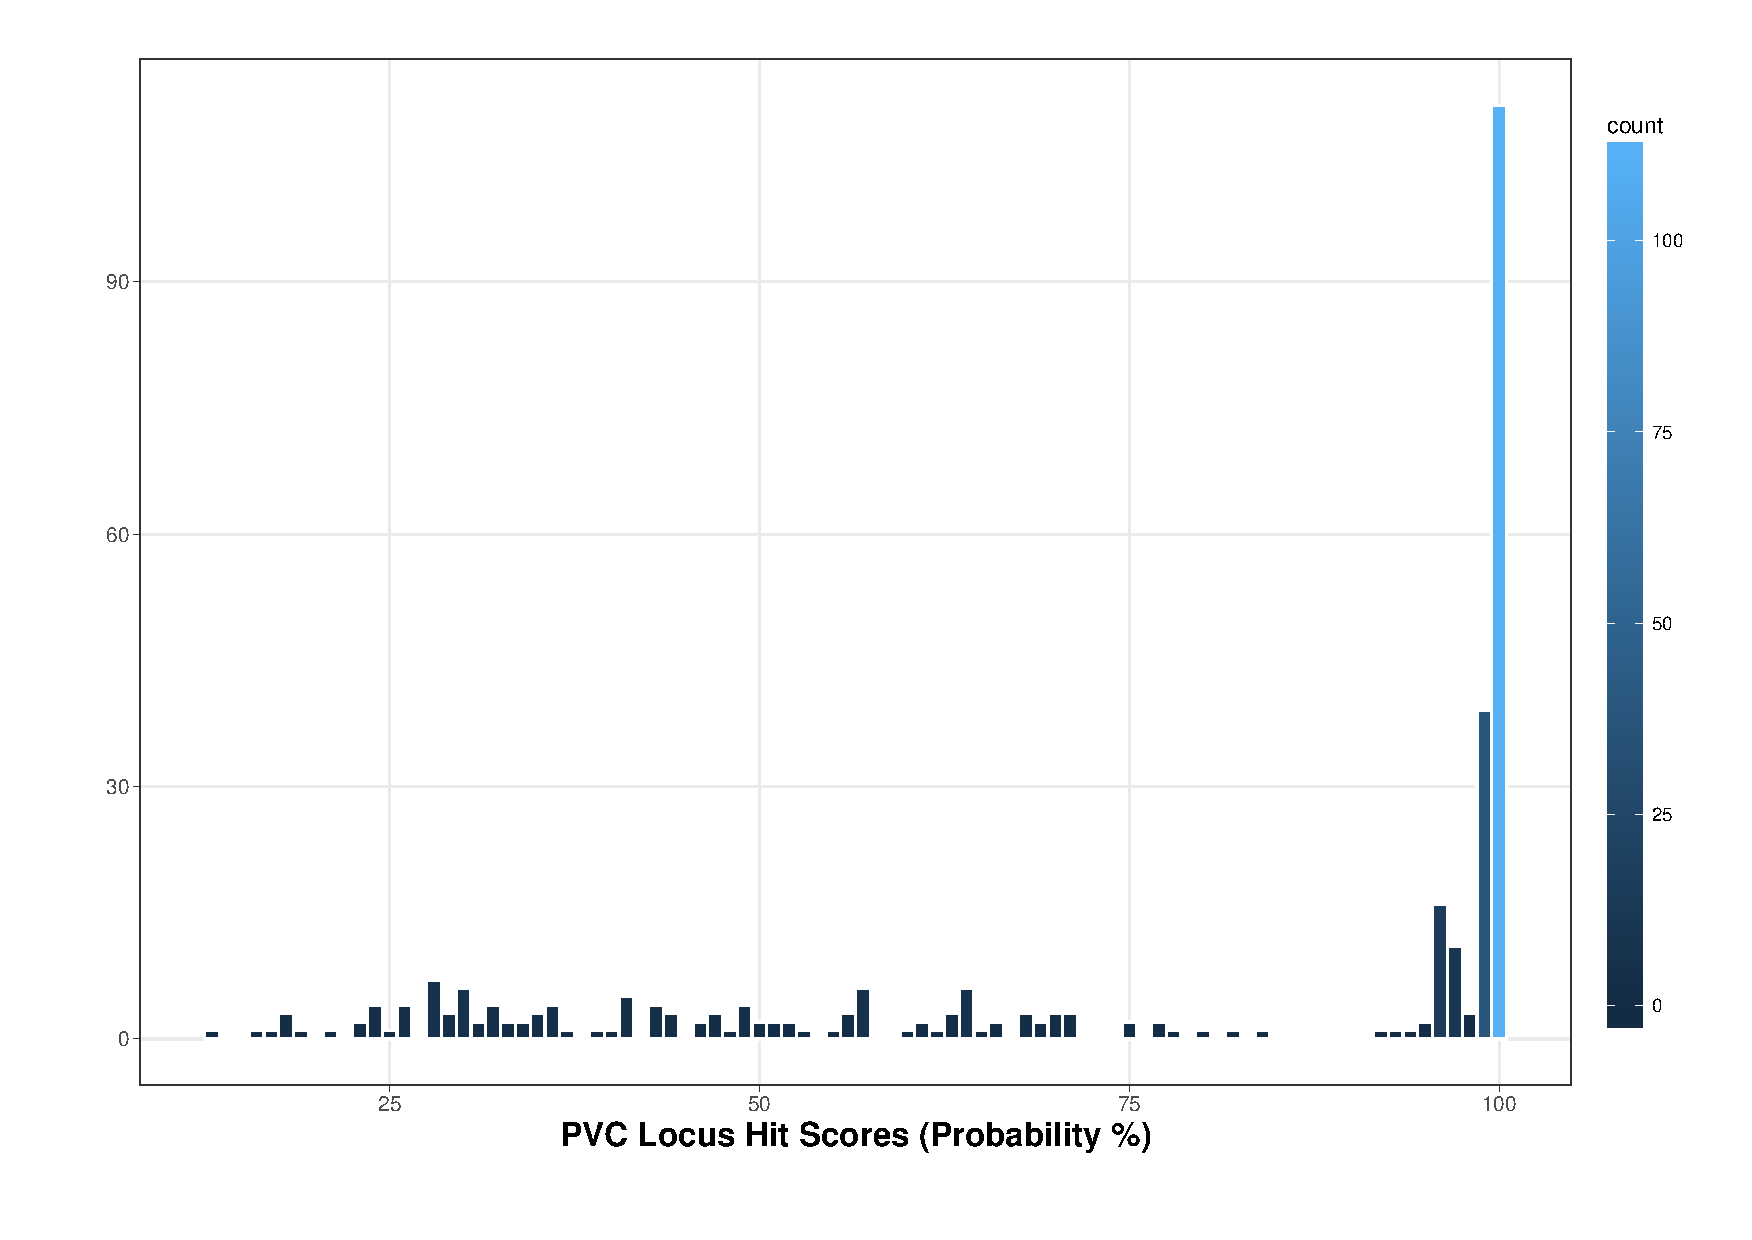
\includegraphics[width=0.9\textwidth]{/Users/joehealey/Documents/Warwick/PhD/Thesis/chapters/chapter3/img/Probabilities.pdf}
	\captionsetup{singlelinecheck=off, justification=justified, font=footnotesize, aboveskip=10pt}
	\caption[HHPred orthologue match scores]{\textsc{\normalsize Distribution of match probabilities for PVC proteins.}\vspace{0.1cm} \newline A histogram of the ``Probability" score for approximately 300 PVC protein sequences. Bars are coloured according to the bin density. Around half of all the proteins are well profiled in this manner, with Probability scores over 80\%. The remaining proteins are distributed widely with a number of examples of proteins which remain with low scores and little to no informative matches.}
	\label{probhist}
\end{figure}


\subsubsection{Homology modelling, threading and structural refinement}
Protein structure modelling was performed using a local installation of the I-Tasser pipeline, on 12 virtual machines \citep{Yang2014, Roy2010, Zhang2008}. I-Tasser was chosen as it generates full length models (whereas some tools only produce models for regions adequately represented by sequence homology), and because it takes a somewhat hybrid approach to modelling, using threading templates, but also \emph{ab initio} molecular dynamics steps for modelling regions (or whole sequences) with no reliable sequence templates, and for final model refinement. I-Tasser is consistently ranked as one of, if not the best, modelling servers/algorithms in the international Critical Assessment of Structure Prediction competitions \citep{Moult2015}.

In most cases, I-Tasser returns 5 models (though sometimes only 1 if the models converge well). Where multiple models were produced, in all upcoming analyses and images the model with the lowest RMSD to the PDB entry identified as closest via HHPred is used. \vref{rmsdhist} shows the distribution of RMSD values obtained from the simulations matched to these structures. The majority of the simulations were able to score well against deposited structures, potentially providing useful analyses.

\begin{figure}[h]
\centering
\thisfloatpagestyle{IHA-fancy-style}
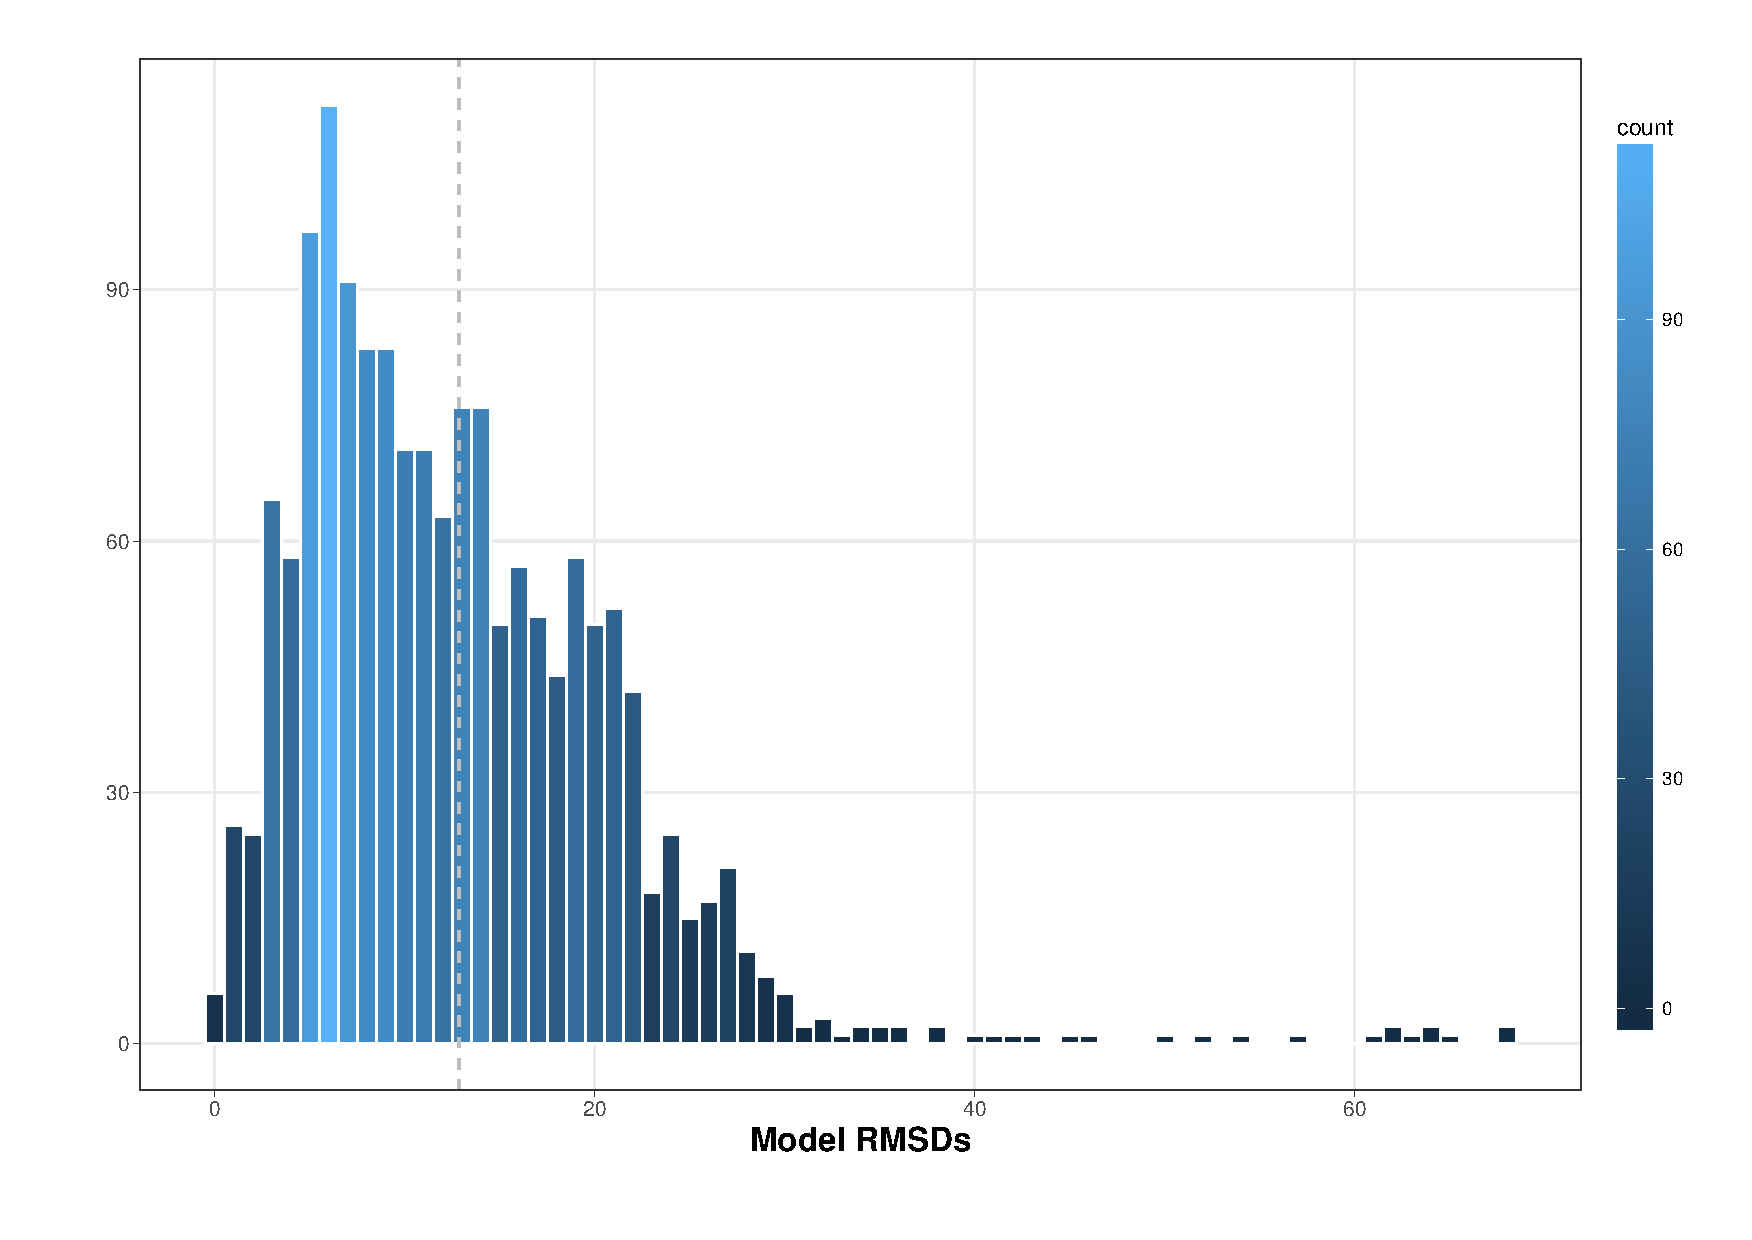
\includegraphics[width=0.9\textwidth]{/Users/joehealey/Documents/Warwick/PhD/Thesis/chapters/chapter3/img/RMSDhist.pdf}
	\captionsetup{singlelinecheck=off, justification=justified, font=footnotesize, aboveskip=10pt}
	\caption[I-Tasser model accuracy distribution - RMSD]{\textsc{\normalsize Distribution of atomic deviations for all simulated models.}\vspace{0.1cm} \newline A histogram of the Root Mean Square Deviation (in \AA{}ngstroms), between a modelled sequence and its closest structural match, as determined by HHSuite. RMSDs were calculated using the MatchMaker function within UCSF Chimera. Reasonable/useful RMSDs of less than $\approx$10 \AA{} are obtained for a significant proportion of the loci simulated. Bars are coloured according to the bin density.}
	\label{rmsdhist}
\end{figure}

That said, despite being the most widely used metric, RMSD is not a perfect measure of structure similarity, as it is prone to large RMSD values (indicative of poor fits) if just a few localised regions are not well matched, even if the protein overall shares similar topology. To this end, I-Tasser also produces calculations of "C-score" (confidence score) and ``TM-score" (template modelling score) \citep{Zhang2005}. I-Tasser provides additional data to assess the best models produced during its molecular dynamics steps, such as the cluster density, which represents the number of times a model passes through a region of 3D modelled space during its molecular dynamics trajectories. Thus the 3D space which is samples most often is likely to represent the conformation of the most favourable models.

\begin{figure}[p]
\centering
\thisfloatpagestyle{IHA-fancy-style}
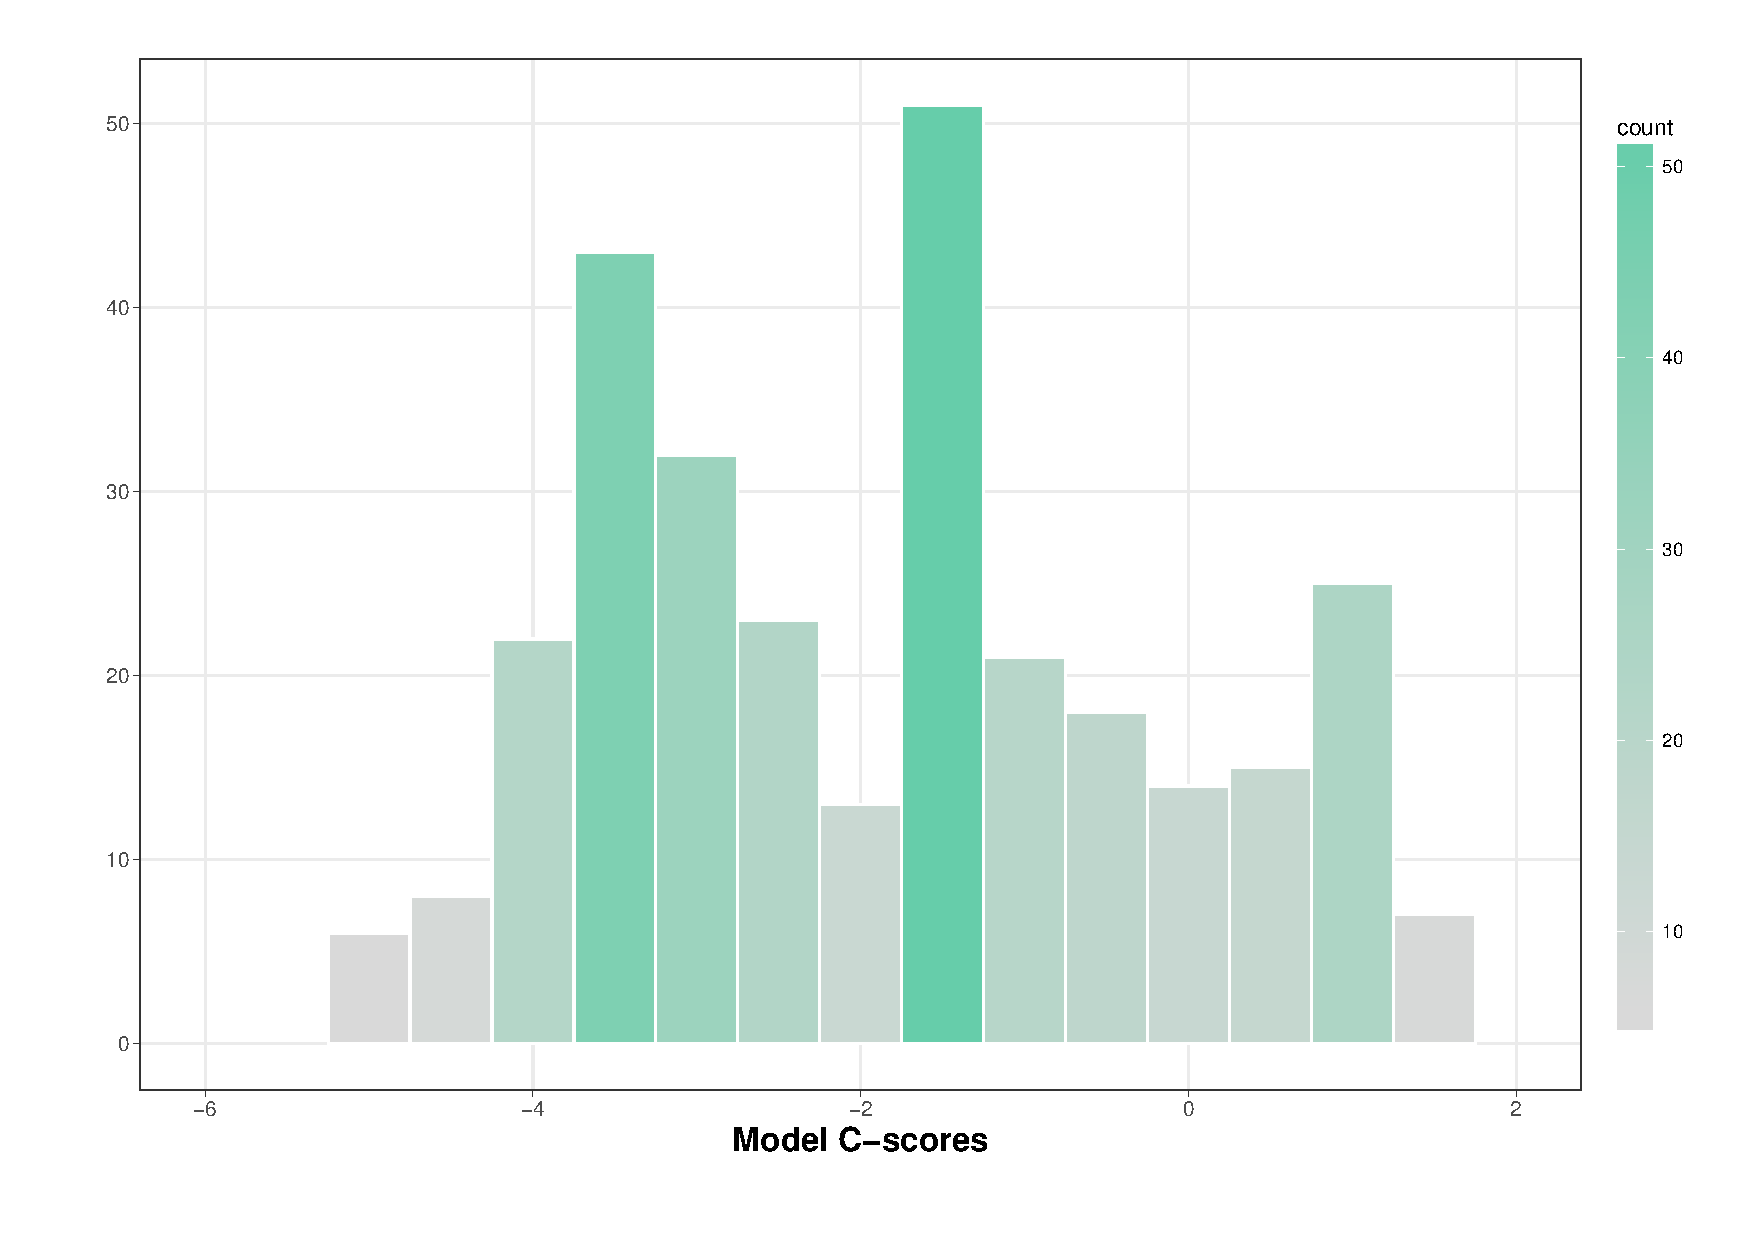
\includegraphics[width=0.9\textwidth, trim={0 30 0 10}, clip]{/Users/joehealey/Documents/Warwick/PhD/Thesis/chapters/chapter3/img/cscores.pdf}
	\captionsetup{singlelinecheck=off, justification=justified, font=footnotesize, aboveskip=7pt}
	\caption[I-Tasser model accuracy distribution - C-score]{\textsc{\normalsize Distribution of the ``C-scores" for all simulated models.}\vspace{0.1cm} \newline A histogram of the ``C-score" from I-Tasser. The C-score is a confidence score calculated internally by I-Tasser based on its confidence in the threading template alignments and convergence of the models. To a rough first estimation, C-scores of greater than approximately -2 indicate reasonable confidence. Approximately half of the models produced therefore have acceptable scores.}
	\label{cscorehist}
\end{figure}
\begin{figure}[p]
\centering
\thisfloatpagestyle{IHA-fancy-style}
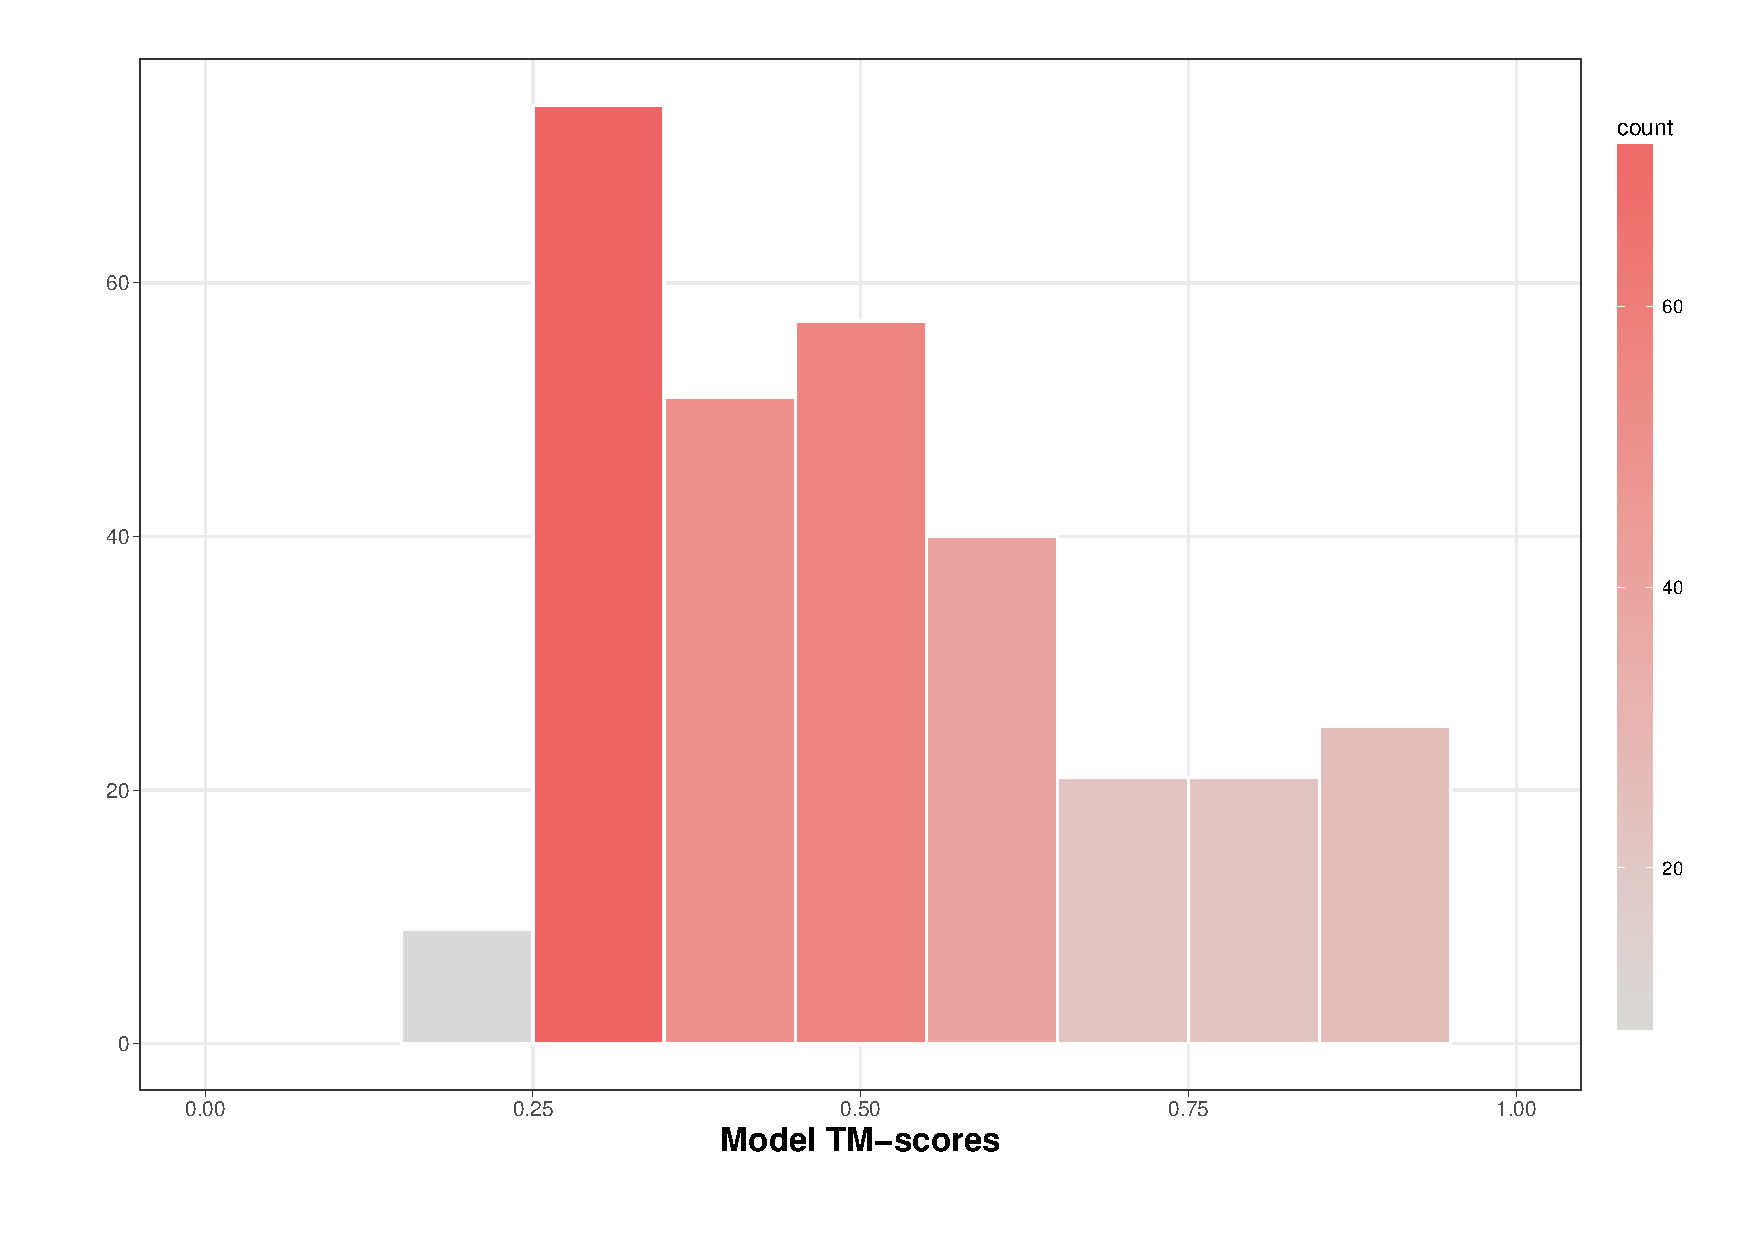
\includegraphics[width=0.9\textwidth, trim={0 30 0 10}, clip]{/Users/joehealey/Documents/Warwick/PhD/Thesis/chapters/chapter3/img/TMscores.pdf}
	\captionsetup{singlelinecheck=off, justification=justified, font=footnotesize, aboveskip=7pt}
	\caption[I-Tasser model accuracy distribution TM-score]{\textsc{\normalsize Distribution of Template Modelling score for all simulated models.}\vspace{0.1cm} \newline A histogram of the TM-score, between a modelled sequence and its closest structural match. TM-scores reflect how well 2 structures match globally, with less susceptibility to local deviations affecting overall score. The vast majority of protein models have TM-scores of greater than 0.25, an acceptable if slightly generous lower bound.}
	\label{tmscorehist}
\end{figure}

There are a large number of models with TM-scores of just over 0.2, (TM-score is in the interval $[0,1]$), which is considered the lower bound on a plausible match between structures \citep{Zhang2005}, suggesting that these protein structures may be of somewhat dubious quality. Roughly half of all modelled proteins have TM scores greater than 0.5 however, and these structures are therefore likely extremely well modelled. This correlates well, as expected, with the C-scores, where higher scores are indicative of better models. C-score is particularly useful when distance based metrics like TM-score and RMSD cannot be used, namely in situations where a template protein could not be identified at all.

It is important to mention however, that despite all these metrics, whether or not a model is useful depends heavily on the question at hand, since models which diverge from the reference structures may still have important/useful information in. Moreover, not all of the metrics correspond perfectly with one another (for instance, some models which have poorer C-scores, actually have good RMSD values. As the epigraph at the start of this chapter suggests, there is no substitute for visually inspecting the models oftentimes, and many of the models are visualised in the remainder of this chapter.

11 of the sequences attempted failed to simulate. Firstly, 8 sequences from the \Pasy{} Kingscliff genome failed to simulate due to the presence of ambiguous amino acids as a result of a lower quality genome assembly. Three proteins were rejected due to being too long - I-Tasser's algorithms have a hard cut-off of 1500 amino acids. 


\subsection{Exploration of the structure of PVCs by functional unit}
%It has been made abundantly clear that it is insufficient to consider sequence similarity alone when comparing structural proteins. Sequences are at liberty to diverge, and if the structure they give rise to is particularly robust, the `space' that the sequence has to drift in is even larger. This is a generally observed phenomenon, but appears to be particularly true for many of the proteins in contractile tail structures. One postulate for this is that phage represent an extremely ancient domain of life, and spend a significant amount of their life cycle outside of the protective environment of the cell they infect. Thus their proteins have evolved over aeons to become particularly stable and robust. The arms race associated with infection cycles has also no doubt driven the diversification of these proteins in an effort to avoid immune mechanisms of their hosts. It has been observed many times in the related literature that, for example, the vgrG/gp5-gp27 spike complex of these caudate systems look almost identical structurally, with many of the same domains identifiable such as the OB-fold, yet may share as little as 12\% protein sequence identity, and due to the slower evolution of proteins sequences attributable codon redundancy, the corresponding DNA sequences may be even less similar.
%
%Consequently, we must make efforts to study the structure as best as possible. In silico methods are improiving all the time, and with more computer power than ever, simulations are becoming routinely feasible. threading approaches are not ideal as they are still too dependent on first identifyin sequence similarity. ab initio approaches allow the structures to be refined without a dependence on the sequence, which should offer an improvement. Structurally conserved proteins with a high degree of robustness should therefore naturally coalesce toward the same structure.

\subsubsection{The PVC tube}
\begin{figure}[h!]
\thisfloatpagestyle{IHA-fancy-style}
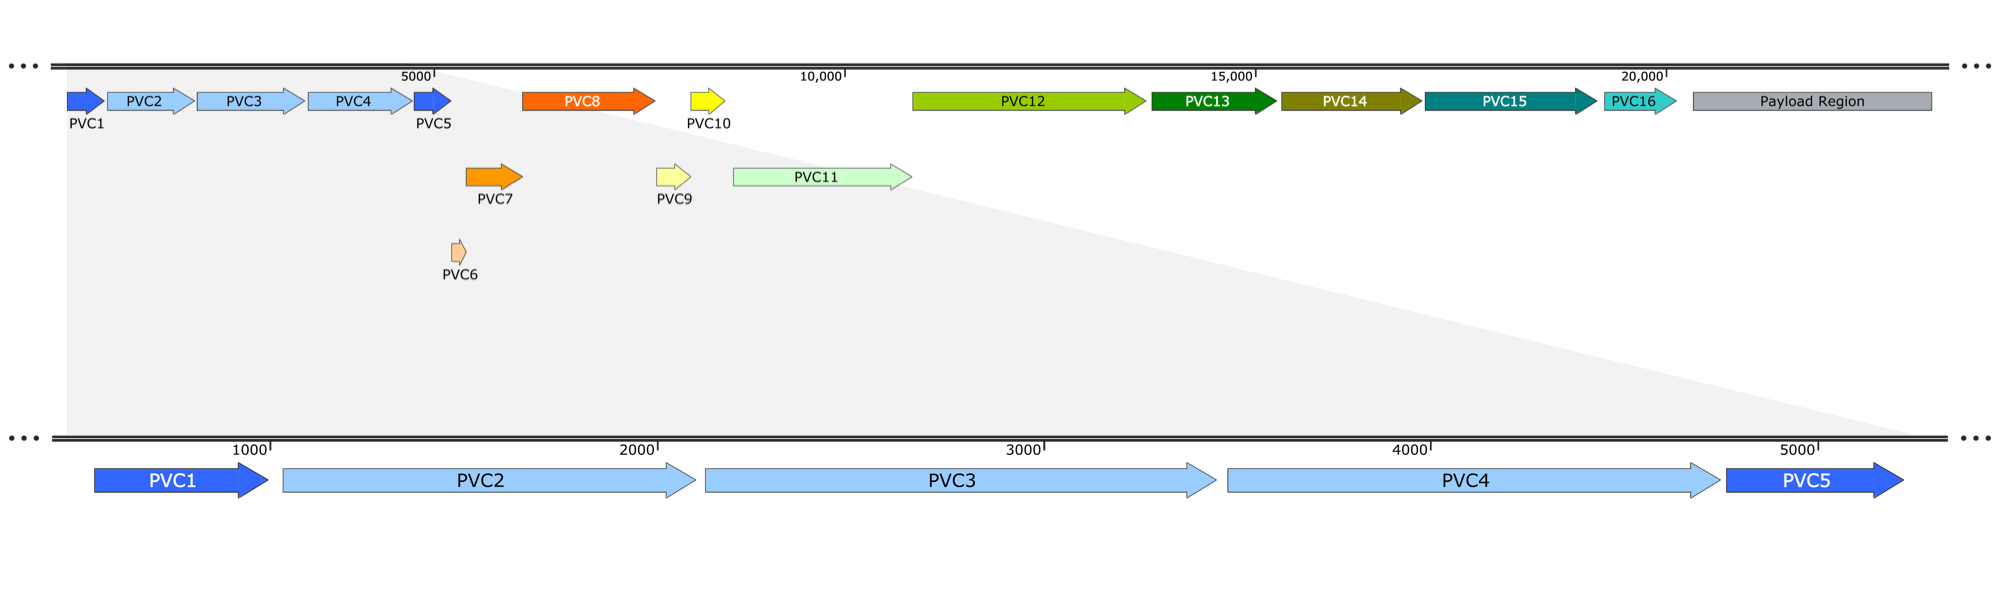
\includegraphics[width=\linewidth]{/Users/joehealey/Documents/Warwick/PhD/Thesis/chapters/chapter3/img/PVC1-5_expanded_map.png}
	\captionsetup{singlelinecheck=off, justification=justified, font=footnotesize, aboveskip=10pt}
	\caption[Tube protein region of a PVC operon]{\textsc{\normalsize The 5 loci that comprise the tube structure of a PVC.}\vspace{0.1cm} \newline The Pnf operon is used as an exemplar of the numbering of loci within an archetypal PVC operon, and 3 colourings are used to demarcate the `functional units' of an operon: blue - tube proteins, orange/yellow - spike complex proteins, green/cyan - the operon `core'. The 5 loci that give rise to the functional unit of the spike complex itself are blown up below as an aid to understanding the operon organisation and the proteins under discussion.}
	\label{PVC1-5map}
\end{figure}


Among the better annotated genes at the outset of this work, the first 5 loci of the PVCs, are predicted to match phage tail tube proteins of various sorts, though the existing annotations were not much more informative than this (for the rest of the operon the vast majority of which were ``hypothetical proteins"). With further inspection, these genes have become consistently annotated as T4-like virus tail tube or baseplate proteins (orthologs of gp6/gp19) and sheath proteins from the recently resolved \emph{Pseudomonas aeruginosa} R-type pyocin. In some previous rounds of annotation, homologies to the Type 6 Secretion Systems of \emph{Edwardsiella tarda}, \emph{Vibrio cholerae}, and \emph{Burkholderia pseudomallei} were also detected for the inner sheath proteins (PVC1 \& 5), which underscores the original notion that PVCs seem to resemble a sort of hybrid, somewhere between a T6SS and a phage in sequence similarity.

From the resolved structure databases and literature, gp19 is known to be the inner sheath of the T4 bacteriophage (as can be seen in PDB IDs 5IV5 and 5W5F \citep{Taylor2016, Zheng2017}), and the outer sheath of PDB ID 3J9Q which corresponds to the resolved pyocin tube structure \citep{Ge2015a}. Over several iterations of homology searches with the HHpred suite, these 3 recent PDB depositions have come to be the most highly similar structures predicted.

\vref{tubehomologs} shows a summarised selection of the orthologues which HHPred has picked up over time. A full list of the most recent orthologies detected can be found in Appendix \vref{structural_appendix}.

\scriptsize
\rowcolors{2}{gray!10}{white}
\begin{tabularx}{\textwidth}{
>{\centering\arraybackslash} m{0.11\textwidth}
>{\centering\arraybackslash} m{0.11\textwidth}
>{\raggedright\arraybackslash} X
>{\raggedright\arraybackslash} X
}
\hiderowcolors
\captionsetup{singlelinecheck=off, justification=justified, font=footnotesize, belowskip=5pt}
\caption[HHPred hit summary for PVC1-5]{\textsc{\normalsize HHPred orthology summary for the tail tube proteins.}\vspace{0.1cm} \newline A summary of homology matches via HHPred for the first 5 PVC loci. The hits have varying degrees of confidence but have Probabilities greater than 60\% and E-Values of less than \sn{1}{-5}. They represent a `collapsed' set of common hits from all the variants for each locus. Hit scores for the inner sheath proteins (PVC1 and 5) are consistently lower than for the outer sheath proteins (PVC2-4) - all scores for the most recent analysis can be found in Appendix \vref{structural_appendix}.}\\
\label{tubehomologs}\\
Locus & PDB ID Hit & Structure & Component \\
\hline\hline
\showrowcolors
\hline

\rowcolor{white!10}                              & 5IV5 & Bacteriophage T4 & Baseplate wedge protein (gp6) \\ 
\rowcolor{white!10}                              & 5W5F & Bacteriophage T4 & Tail tube protein (gp19) \\
\rowcolor{white!10}                              & 3EAA & T6SS             & Inner sheath protein (Hcp/TssD)\\
\rowcolor{white!10} \multirow{-4}{*}{PVC1 \& 5*} & 4TV4 & T6SS             & Inner sheath protein (Hcp/TssD)\\
\rowcolor{gray!10}  PVC2, 3, \& 4                & 3J9Q & R-type Pyocin    & Outer sheath protein \\

\end{tabularx}
\hrule
\vspace{0.1cm}
{\tiny \noindent * PVC5 attracts the same 3 homology matches as PVC1, plus 4TV4.}
\normalsize

\vrefrange{PVC1comparisons}{PVC5comparisons} showcases the similarities and differences in structure between the first 5 PVC loci and their nearest structural homologs. In addition, the figure also shows the structure of the R-type pyocin which the outer sheath protein match to so conclusively, to try to understand why the inner sheath proteins do not reflect this same orthology; as well as a simulated structure for the Antifeeding Prophage equivalent locus. The Afp is the closest orthologue when only DNA or amino acid sequence is considered, but no resolved structure exists.

\begin{figure}[h]
 \thispagestyle{augment}
 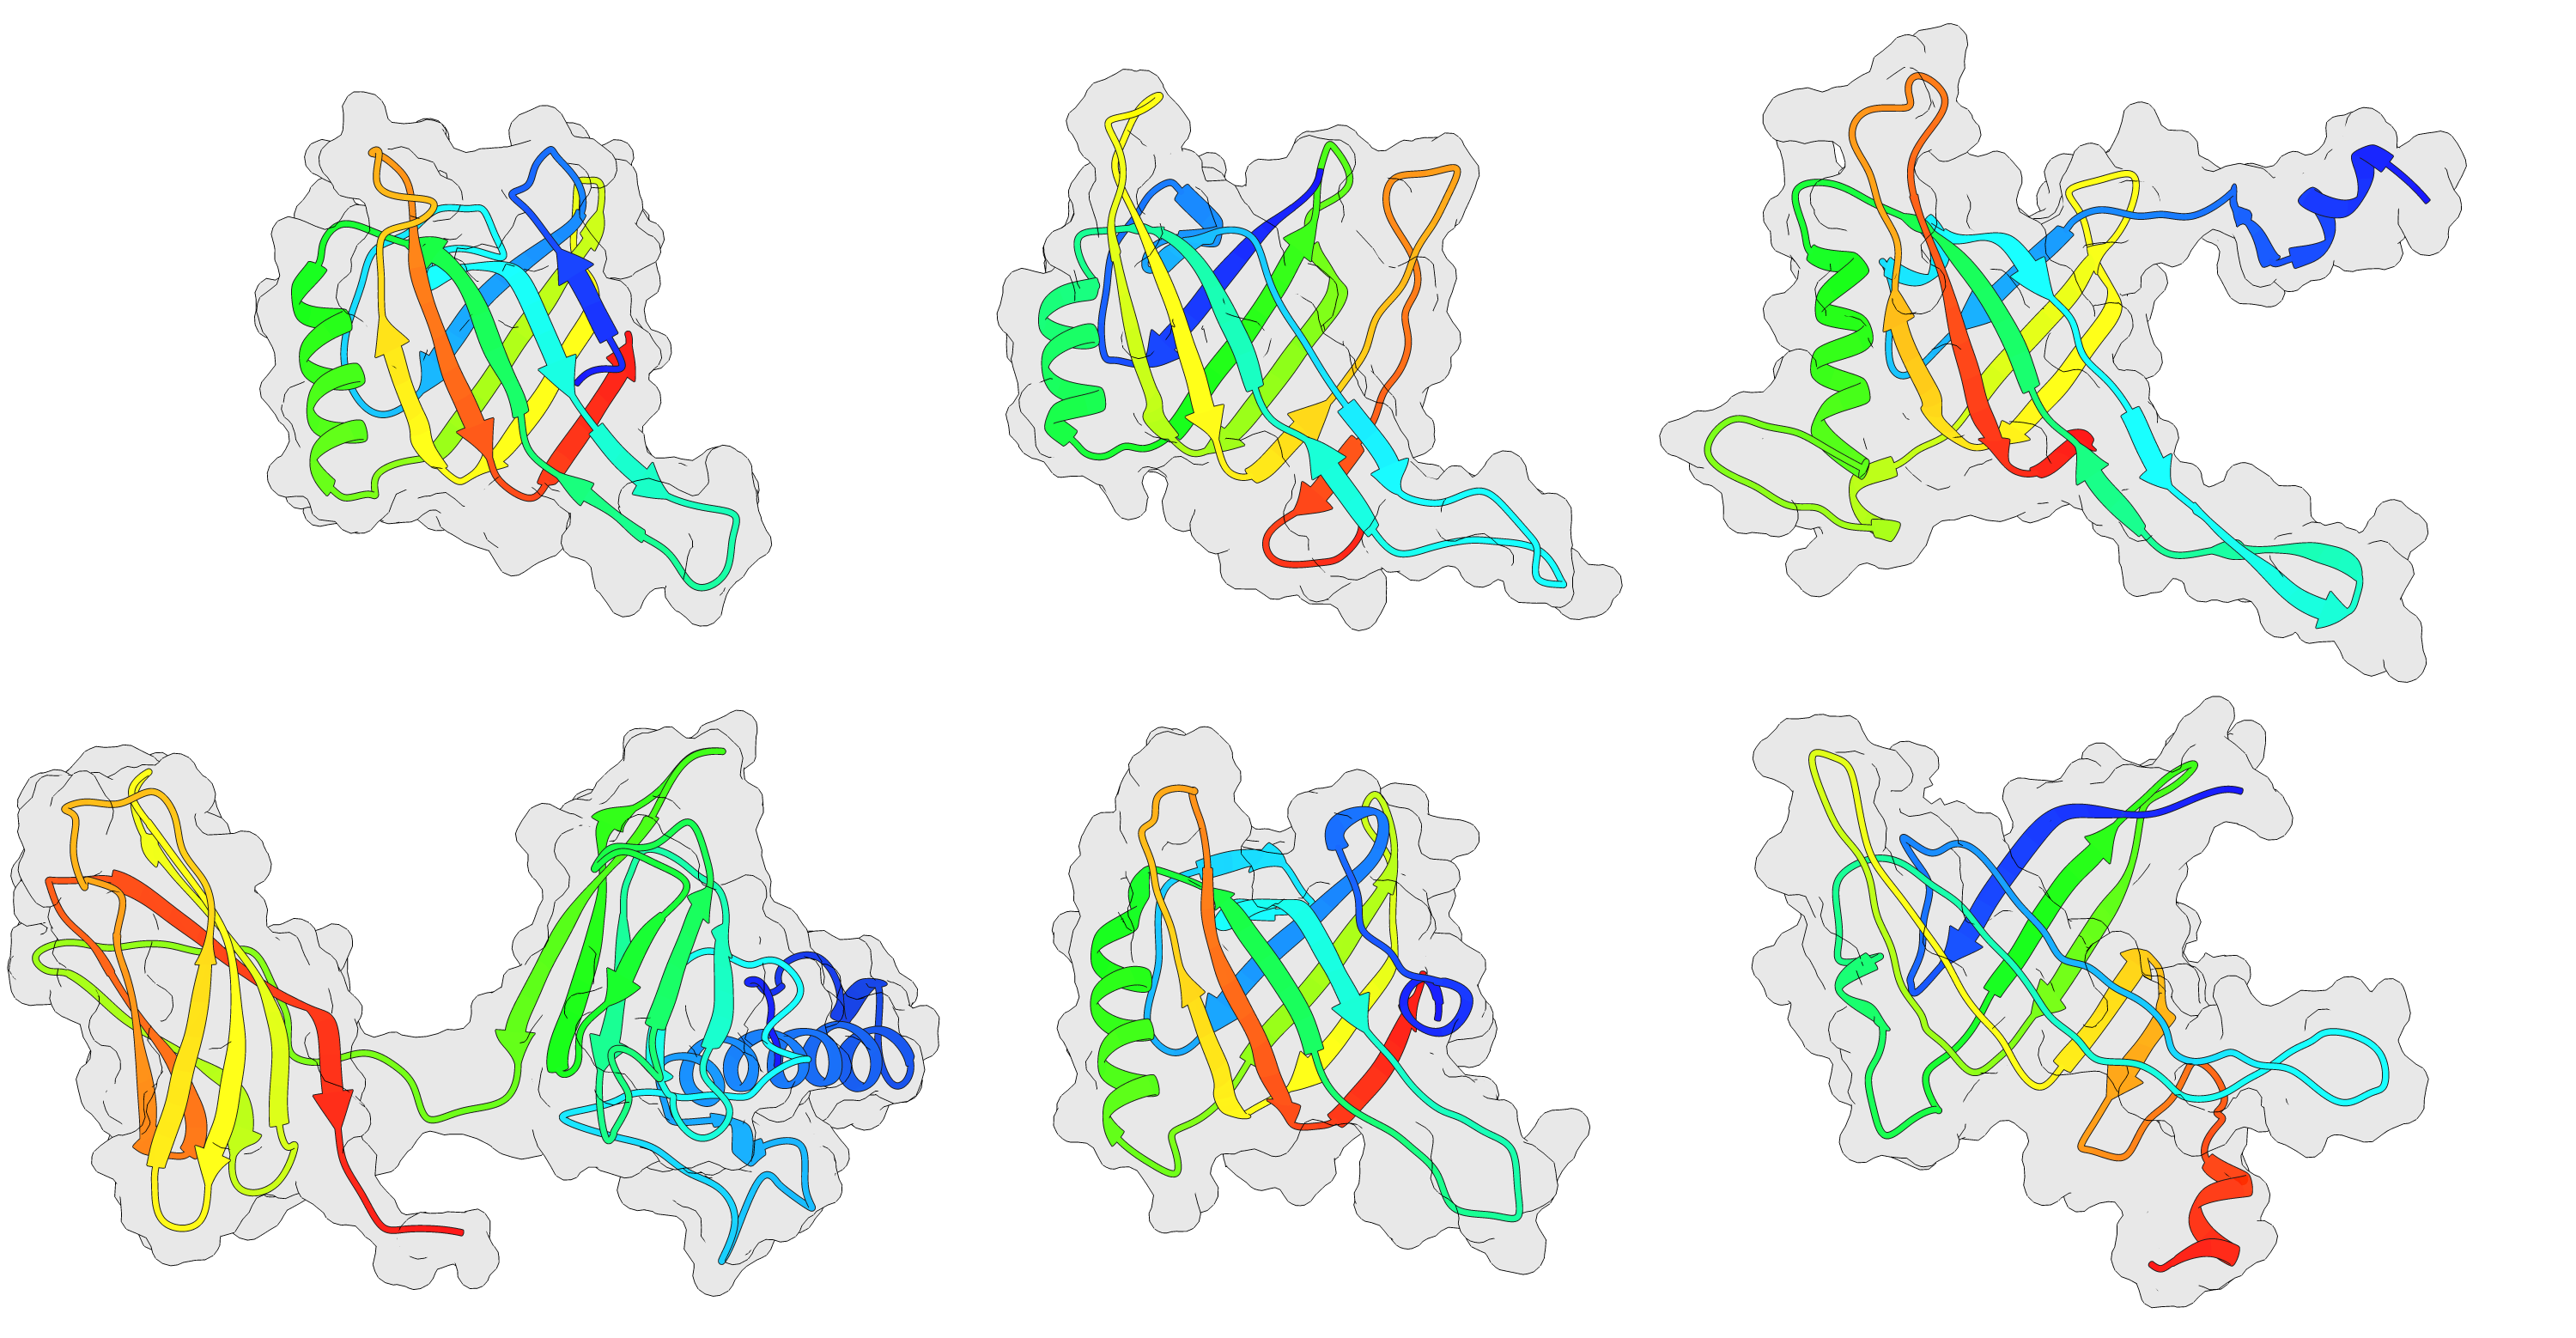
\includegraphics[width=\textwidth, trim={0 0 0 0}, clip]{/Users/joehealey/Documents/Warwick/PhD/Thesis/chapters/chapter3/img/PVC1_homolog_comparison.png}
 \put(-380,108){\small PVC Simulation}
 \put(-227,106){\small T6SS}
 \put(-105,108){\small T4 Tube}
 \put(-374,-10){\small T4 Baseplate}
 \put(-241,-10){\small Afp Simulation}
 \put(-100,-10){\small Pyocin} 
 \captionsetup{singlelinecheck=off, justification=justified, font=footnotesize, aboveskip=20pt}
 \caption[PVC1 homolog comparisons]{\textsc{\normalsize Comparisons of the structure of PVC locus 1 to orthologous proteins.}\vspace{0.1cm} \newline An example model of PVC locus 1 from the PVCPnf operon of \Pasy{} ATCC43949. Here the structure is compared to (from top left to bottom right) the Hcp protein (3EAA) of the \emph{E. tarda} T6SS, gp19 (5W5F chain V) from the T4 bacteriophage, gp6 also from T4 (5IV5 chain F), a simulated Afp1 structure, and an interior sheath monomer from the R-type pyocin (3J9Q chain V). Models are shown `rainbow' coloured, from one terminus to the other, with a molecular surface `ghost'. It is evident that the 2 T4 proteins, despite being frequent sequence based matches to PVC1 (and 5), are not the closest matches in terms of structural conformation. The 3D model to accompany this page shows superimposed $\alpha$-carbon chain traces for all the structures (though without the T4 baseplate as its superposition is poor) - the PVC protein is rendered in thicker red wires/pipes, and the homologs in various monochrome shades. }
	\label{PVC1comparisons}
\end{figure}

The inner sheath proteins from all these structures form a conserved pair of anti-parallel $\beta$-sheets which are sandwiched together approximately perpendicular to one another (with the exception of the T4 baseplate protein which is clearly an erroneous homology). They all exhibit a lower right hand extension positioned almost exactly in the centre of the amino acid chain (cyan/aquamarine). In the case of the T4 gp19 tube protein, this is quite extended, along with a much longer protruding C-terminus (dark blue).

The PDB ID 5IV5 is the entire baseplate complex, including part of the tube (which is PDB ID 5W5F), from the T4 phage. It seems unusual that many of the proteins match (at the sequence and secondary structure level) so well to chains within the model which are \emph{not} the tube, instead forming part of the baseplate complex, primarily gp6. It is clear from looking at the structures visually that these proteins are homologues of the inner sheath proteins (which are matched by HHPred for some of the PVC1 proteins, but the minority in actual fact - see \vref{HHpredPVC1}). The basis for matching the gp6 monomer, therefore, is likely because they share similar predominantly $\beta$-sheet secondary structures (ADD SOMETHING ABOUT THEIR SEQUENCE IDENTITY - CAN'T BE THE EXPLANATION?).

The T4 gp6 protein (modelled here is chain F from 5IV5) has some extended loops which would interface with the neighbouring monomers compared with both the PVC model and Hcp protein (PDB ID 3EAA). 

Strangely, it wasn't easy to obtain good quality overlays when matching chains between the PVC models and those of the R-type pyocin, even though they visible resemble one another reasonably well, and could be imposed within each other's simulated density maps well (not shown). To this end, some manual rotation/translation of the model has been performed to have a consistent orientation with the other models.

Electrostatic comparisons of interior tube proteins + general comparisons
PVC1 vs Hcp vs gp19 vs R-type pyocin (also show their pairwise sequence identities?)

comparisons of PVCs2,3,4 to try and understand their paralogy? Same with PVC 1 and 5
Compare the structures of the MOST different PVC1s, PVC5s, etc.

Might some PVCs be defunct? If not - is there a minimal outer sheath?

Measurements of the axes of the tube proteins to extrapolate PVC length and subunits.


\myparagraph{Understanding operon paralogy in structural genes by examining structural conservation}
An unanswered question is why \emph{Photorhabdus} has managed to maintain so many copies of what appear to be highly paralogous proteins in the tube region. Not only are the proteins paralogous within a single operon, but multiplied up by 5 or 6 times to account for the other operons, and somehow proteins with as many as 10 or more copies are somehow preserved. If the proteins are sufficiently different in specific ways, it may be the case that they aren't so paralogous after all. 


To highlight the similarities and differences between loci from different PVCs, to highlight the variability between operons, the structures are also rendered by conservation by overlaying the multiple sequence alignments in \ref{bioinformatics_appendix}. 

PVC5 matched additional orthologues that PVC1, did not - let's explore the differences between PVC1 and 5

\cite{Hurst2004} demonstrated that Afp2 is required for formation of a toxic Afp. In several PVC operons a deletion in one of the 3 proteins which match to outer sheaths are observed. Initially, it was not obvious which of these 3 proteins, assumed to be equally paralogous, would be deleted in each case. It seemed unusual that 3 outer sheath CDSs would be required whilst only 2 inner sheath CDSs are ever present, if stoichiometry was the only explanation for their paralogy. On further inspection, it appears that the deletions in these outer sheath proteins is always PVC3 rather than 2 or 4. Unpublished communication from the Hurst lab has proposed that PVC4 may actually be a slightly modified variant of the outer tube. This may be such that it functions as an adapter protein at one end of the tube, possibly as a collar that interfaces with the baseplate.


It is also interesting that the inner and outer tube orthologies do not share the same provenance. It might be expected that they should all match to the next closest structure (e.g. all matching to the \emph{P. aeruginosa} R-type pyocin). This indicates that the inner and outer sheaths may be subject to different evolutionary pressures. Additionally, interior sheath proteins are smaller and better conserved. This may, therefore, be indicative of \emph{Photorhabdus} honing the exterior of the sheath in different environments. An appealing hypothesis, especially since legacy data has shown that different PVCs are deployed in very particular inducing conditions\todo{move to discussion?}.



\addfloat{EM density fittings for AFP/T4/PVC sheaths etc}



PVC6 translationally coupled to PVC5, maybe a role in the tube itself then?
	- Could PVC5 be a special homolog which forms an adapter, similar to PVC4 potentially?

Homology to gp6 is likely spurious? Show that they fit gp19 and other inner sheath proteins better (reinforces the argument that sequence alone is not enough).






\subsubsection{The spike complex}
\begin{figure}[h!]
\thisfloatpagestyle{IHA-fancy-style}
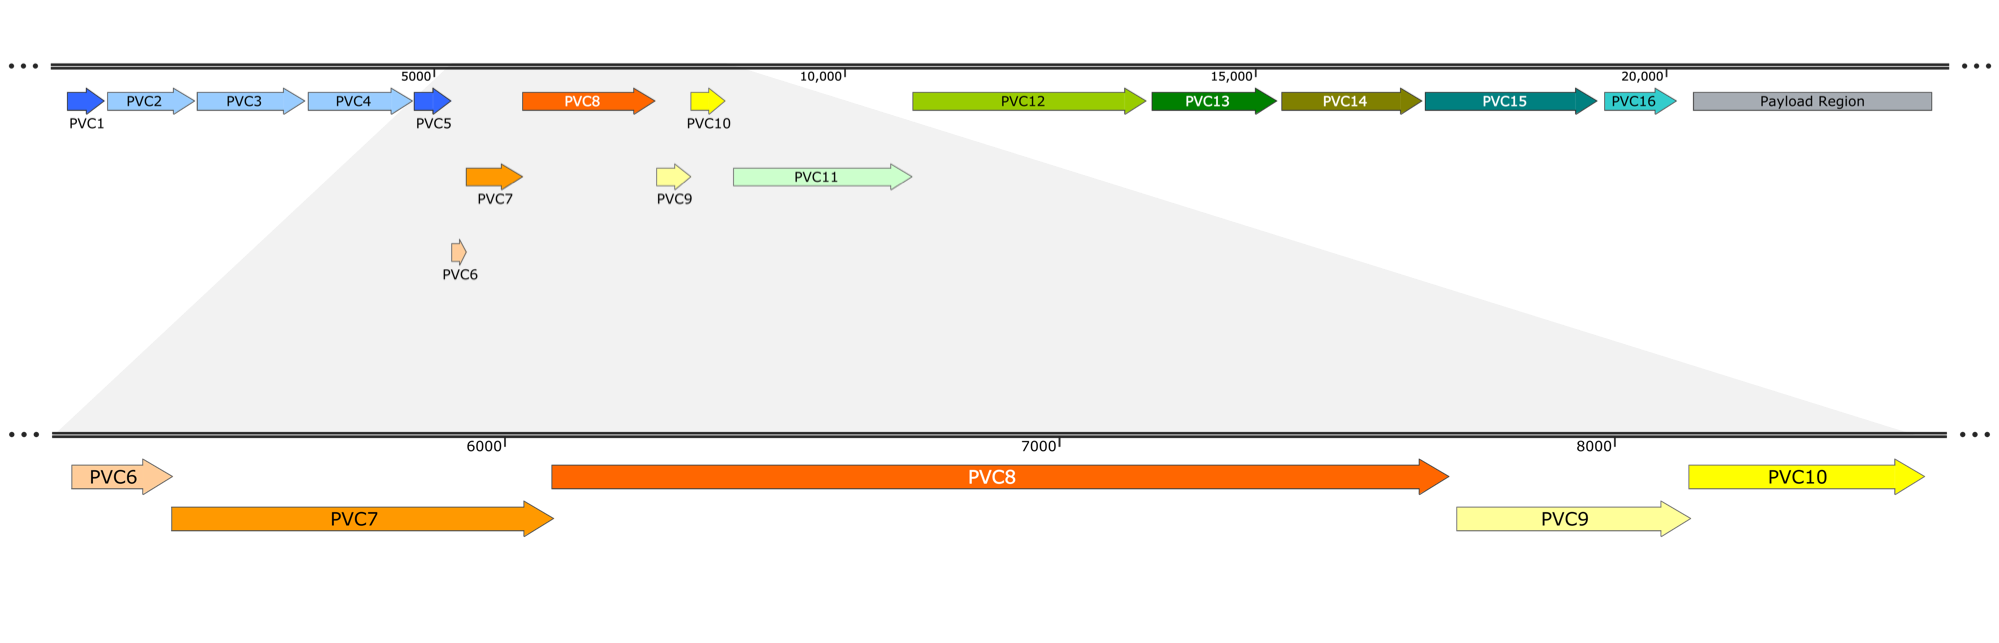
\includegraphics[width=\linewidth]{/Users/joehealey/Documents/Warwick/PhD/Thesis/chapters/chapter3/img/PVC6-10_expanded_map.png}
	\captionsetup{singlelinecheck=off, justification=justified, font=footnotesize, aboveskip=10pt}
	\caption[Spike complex protein region of a PVC operon]{\textsc{\normalsize The 5 loci predicted to comprise the spike and baseplate complex of a PVC.}\vspace{0.1cm} \newline The Pnf operon is used as an exemplar of the numbering of loci within an archetypal PVC operon, and 3 colourings are used to demarcate the `functional units' of an operon: blue - tube proteins, orange/yellow - spike complex proteins, green/cyan - the operon `core'. The 5 loci that give rise to the functional unit of the spike complex itself are blown up below as an aid to understanding the operon organisation and the proteins under discussion.}
	\label{PVC6-10map}
\end{figure}


Comparisons of VgrGs - show that the lysozyme domain looks to me missing compared to T4. Maybe explains the gene next to it?

PAAR models. Vaguely similar in shape, known to be super variable so difficult to spot via sequence identity.

\subsubsection{The operon core}
\begin{figure}[h!]
\thisfloatpagestyle{IHA-fancy-style}
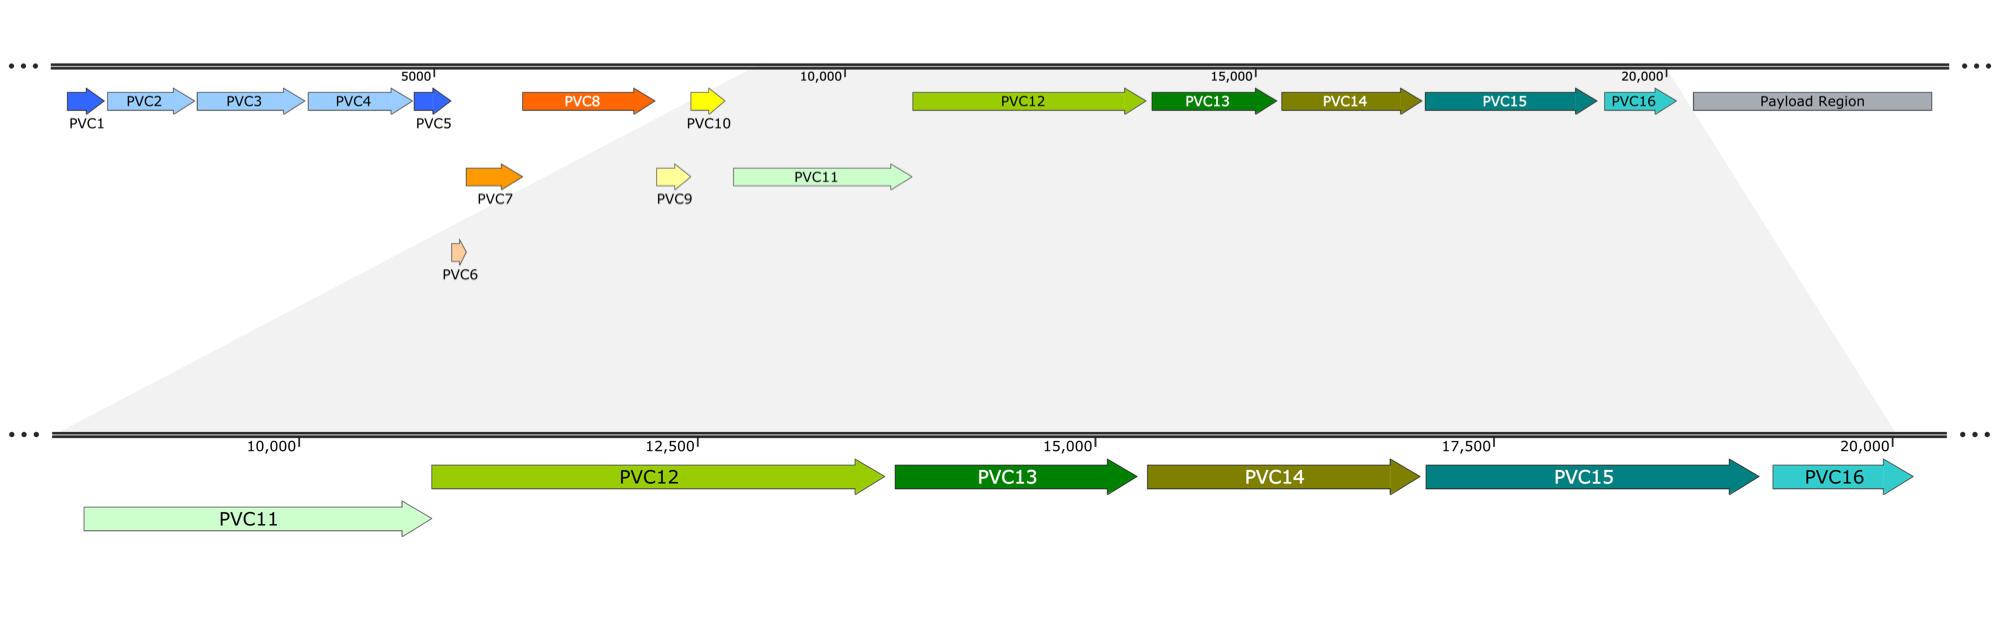
\includegraphics[width=\linewidth]{/Users/joehealey/Documents/Warwick/PhD/Thesis/chapters/chapter3/img/PVC11-16_expanded_map.png}
	\captionsetup{singlelinecheck=off, justification=justified, font=footnotesize, aboveskip=10pt}
	\caption[`Core' protein region of a PVC operon]{\textsc{\normalsize The 6 loci comprising the `core' of a PVC operon with various functions.}\vspace{0.1cm} \newline The Pnf operon is used as an exemplar of the numbering of loci within an archetypal PVC operon, and 3 colourings are used to demarcate the `functional units' of an operon: blue - tube proteins, orange/yellow - spike complex proteins, green/cyan - the operon `core'. The 6 loci that give rise to the operon core are blown up below as an aid to understanding the operon organisation and the proteins under discussion. The `core' is a collection of conserved proteins present in almost all PVC operons, typically comprised of larger, single copy genes, some which are proposed to be structural, but also the proteins responsible for cell surface adhesion, and an ATPase which potentially loads payloads or recycles the tube apparatus.}
	\label{PVC11-16map}
\end{figure}
Tail fibres - highlight hyper variable domains

Tape measure proteins - high in helix? (add the calculations from the hhpred hits).
Tape measure proteins - annotate the MSA with helical regions according to DSSP?
Tape measure proteins - speculate on length

\subsubsection{The payload region}
\addfloat{CDSs in operon position}











\section{Discussion}
PVCs are a hybrid between T4 and pyocin like structures, with an inner sheath most resembling the former, and an outer sheath the latter.

Mention translational coupling of the spike complex and PVC5


\todo[inline]{Table of HHpred results in appendix}
\todo[inline]{Correlation between sequence similarity and structure similarity}

Evaluations/Considerations:
Obviously the simulations presented in this chapter are of assorted qualities, and care must be taken when concluding anything from theoretical data alone, however, there is a sufficient body of related proteins for many PVC loci, that comparative modelling can provide, and has provided, hypotheses and potential answers for a number of questions which are not answerable without resolving the structures either experimentally or otherwise.


